\begin{figure}
\centering
\hspace{-4em}
\begin{subfigure}[b]{0.26\textwidth}
\centering
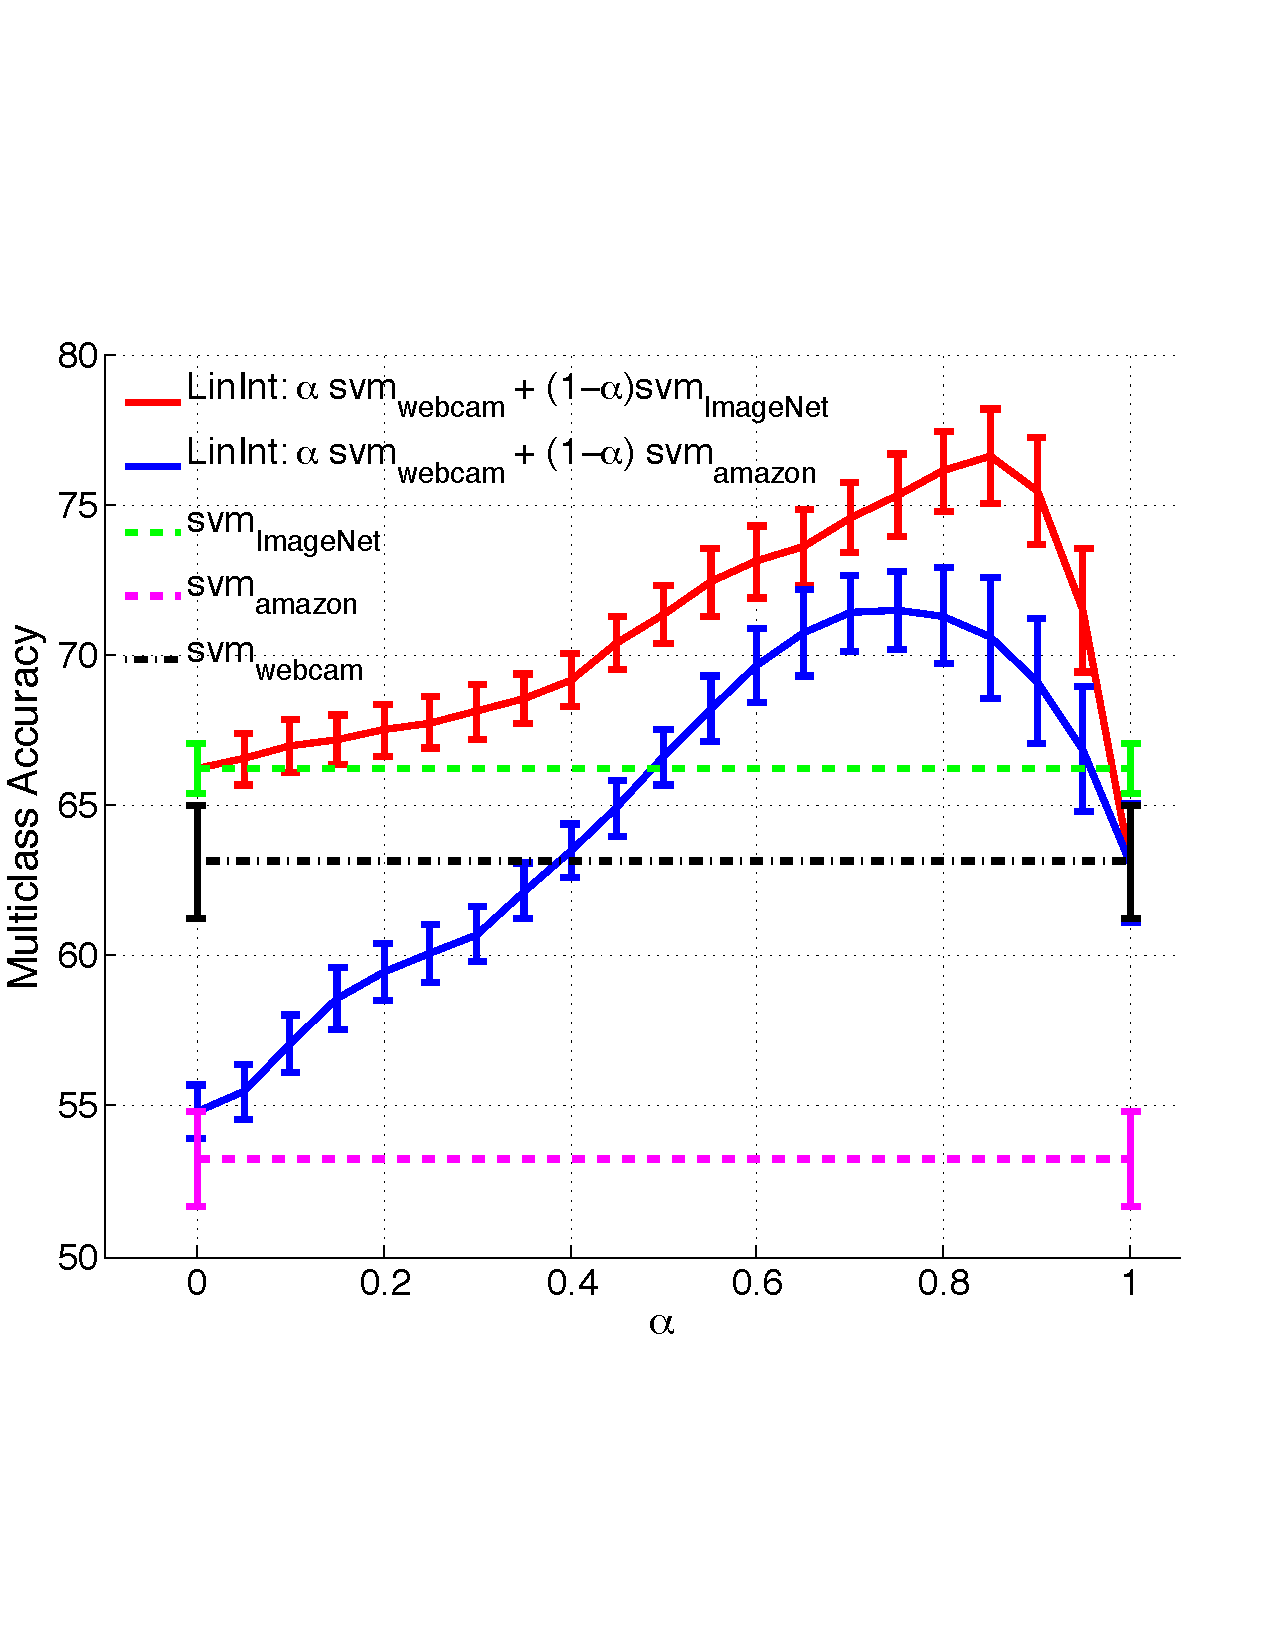
\includegraphics[height=\textwidth]{figs/amazonAndImagenet-linint-vs-alpha_C1_fc8.pdf}
\caption{DLF Parameter $\alpha$}
\label{fig:linint-eval}
\end{subfigure}
%
%\hfill
\hspace{3em}
\begin{subfigure}[b]{0.27\textwidth}
\centering
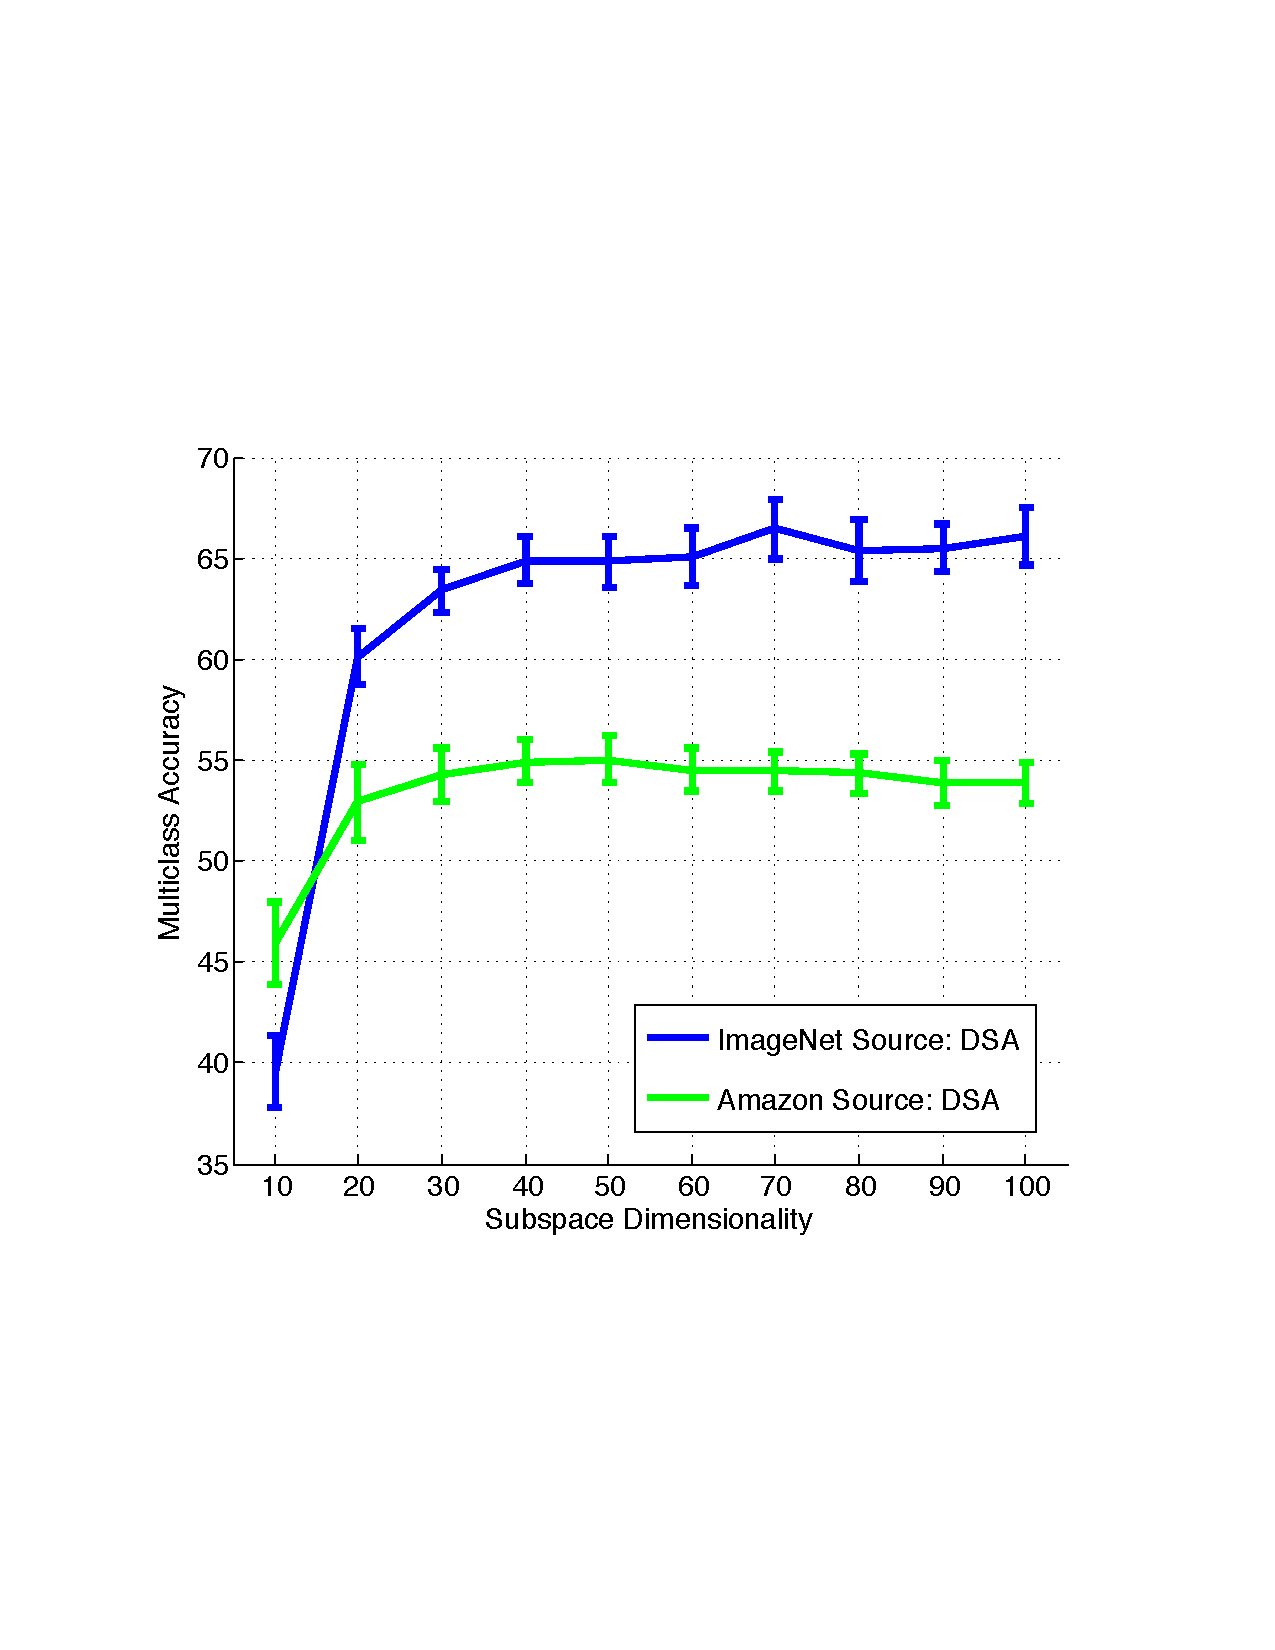
\includegraphics[height=\linewidth]{figs/amazonAndImagenet-sa_dim_C1_fc7.pdf}
\caption{DSA: subspace dimension}
\label{fig:sagfk-eval}
\end{subfigure}
%
%\hfill
\begin{subfigure}[b]{0.28\textwidth}
\centering
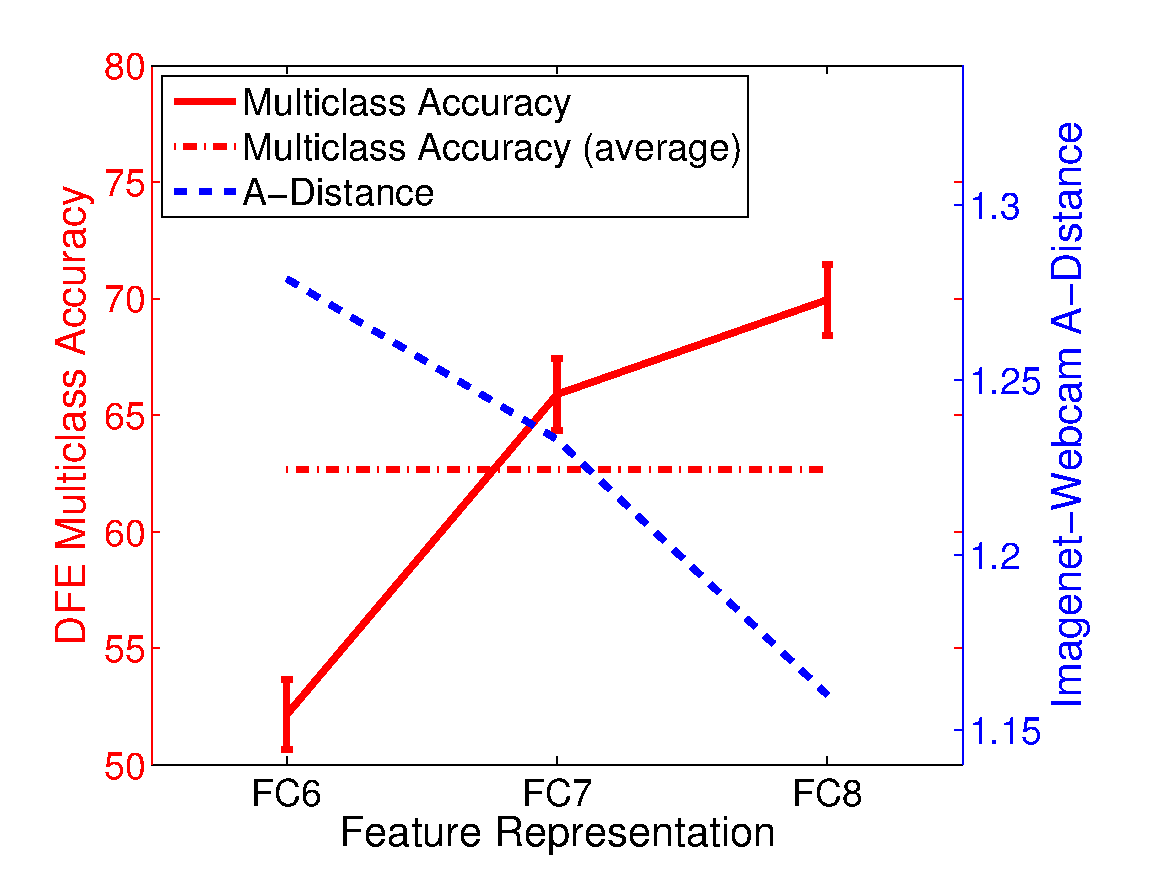
\includegraphics[height=\linewidth]{figs/imgnet_webcam_a_dist_with_avg}
\caption{Layer Selection}
\label{fig:a-dist-eval}
\end{subfigure}
%
\caption{Evaluation of hyperparameters for domain adaptation methods. (a) Analysis of the combination hyperparameter $\alpha$ for Deep Late Fusion (DLF) with linear interpolation: We find that choosing to weight the target domain higher than the source domain performs best.  (b) Analysis of the subspace dimensionality for Deep Subspace Alignment (DSA): The algorithm is not sensitive to the subspace dimension chosen. (c) Analysis of model selection: after which pre-trained layer do we add our adaptation layer: We show that using our layer selection criteria (A-distance) correlates with final classification accuracy.}
\label{fig:hyperparam-eval}
\end{figure}
